\documentclass{article}
\usepackage{graphicx} % Required for inserting images
\usepackage{authblk} % For author affiliations
\usepackage{hyperref} % For hyperlinks
\usepackage[margin=1in]{geometry} % Standard margins
\usepackage{natbib} % For bibliography management
\usepackage{enumitem} % For customising lists
\usepackage{color}
\usepackage{amsmath}
\usepackage{float}
\usepackage{booktabs}
\newlist{tree}{itemize}{10}
\setlist[tree]{label=-}
\setlistdepth{10} 
\usepackage{pdfpages}
\usepackage{pdflscape}
\usepackage{array}
% \usepackage{pdflscape}
\usepackage{longtable}
\usepackage{booktabs}
 \usepackage{colortbl}
\usepackage{color}
 \usepackage{tabularray}
 \newcommand\Fontvi{\fontsize{6}{6}\selectfont}

\renewcommand{\theequation}{S.\arabic{equation}}

\newcommand{\beginsupplement}{%
        \setcounter{section}{0}
        \renewcommand{\thesection}{S\arabic{section}}%
        \setcounter{table}{0}
        \renewcommand{\thetable}{S\arabic{table}}%
        \setcounter{figure}{0}
        \renewcommand{\thefigure}{S\arabic{figure}}%
     }
     
\title{Integrating Multiple Data Sources in Infectious Disease Modelling: Best Practices and Implementation -- Supplementary Materials}

\author{}

\date{}

\begin{document}

\maketitle

\beginsupplement

\section{Full model specification for combining multiple data sources}
The target estimand for this case study is the time-varying reproduction number $R_t$ during the outbreak period. The objective is to illustrate the process of integrating multiple epidemiological data sources. For each case, we consider two main approaches: fitting separate models independently to each data source and combining the resulting estimates, and fitting a joint model that incorporates both data sources simultaneously. Throughout this work, we denote time series of the variable $X_t$ indexed from day 1 to day $T$ by $X_{1:T} = \{X_1, X_2, \ldots, X_T\}$.


\subsection{Case Study 1: Two-source integration (Cases and Deaths)}

\subsubsection{Separate models: Independent estimation from Cases and Deaths}

\paragraph{Case-based $R_{t}$ estimation:}
We model the latent infection incidence $I_{t}$ at time $t$ using the renewal equation framework, considering one of three variants for the infection process model:
\begin{align}\label{latent_inf}
I_t \sim f\big(R_t, I_{1:t-1}\big) =
\begin{cases} 
 & R_t \sum_{s=1}^\infty I_{t-s} w_s, \hspace{2.5cm}\text{or}\\[5pt]
 & \mathrm{Poisson}\!\Big(R_t \sum_{s=1}^\infty I_{t-s} w_s\Big), \hspace{1cm}\text{or}\\[5pt]
 & \mathrm{NegBin}\!\Big(R_t \sum_{s=1}^\infty I_{t-s} w_s,\; k\Big),
\end{cases}
\end{align}
where $w_s$ is the generation time distribution probability mass function, and $k$ is the dispersion parameter.

The observation model relates reported cases $\widehat{I}_{1:T}$ to latent infections as:
\begin{align}\label{obs_inf}
\widehat{I}_t \sim \mathrm{Poisson}\left( \sum_{s=1}^\infty N_{s,t} \right), \quad N_{s,t} \sim \mathrm{TruncatedMultinomial}(I_s, \alpha_{t-s}),
\end{align}
where $N_{s,t}$ is the number of people infected on day $s$ and reported as a case on day $t$, and $\alpha_s$ is the probability that an infection is reported as a case $s$ days after infection. Using observed case incidence $\widehat{I}_{1:T}$, inference targets the posterior distribution:
\begin{align}
p\big(R_{1:T}, I_{1:T}, \theta \,\big|\, \widehat{I}_{1:T}\big),
\end{align}
where $\theta$ denotes all model parameters (e.g., $k$, $\alpha$). This yields posterior estimates $R_{1:T}^{c}$, with the superscript $c$ indicating that this is the reproduction number from case incidence only.

\paragraph{Death-based $R_{t}$ estimation:}
The number of deaths $D_t$ on day $t$ depends on the time series of infections $I_{t}$ generated by the same infection process model as in Eq.~\eqref{latent_inf}, governed by $R_{t}$:
\begin{align}\label{latent_death}
\begin{cases}
I_t \sim f\big(R_t, I_{1:t-1}\big),\\[4pt]
D_t \sim \mathrm{Poisson}\!\Big( p_d \sum_{s=1}^\infty I_{t-s} v_s \Big),
\end{cases}
\end{align}
where $p_d$ is the infection-fatality ratio and $v_s$ is the infection-to-death delay distribution.

Observed deaths data $\widehat{D}_{1:T}$ are related to latent deaths via:
\begin{align}\label{obs_death}
\widehat{D}_t = \sum_{s=1}^\infty M_{s,t}, \quad M_{s,t} \sim \mathrm{Multinomial}(D_s, \beta_{t-s}),
\end{align}
where $M_{s,t}$ is the number of deaths that occurred on day $s$ and were registered on day $t$ and $\beta_s$ the death-to-registration delay distribution.  
Fitting this model to $\widehat{D}_{1:T}$ targets the posterior:
\begin{align}
p\big(R_{1:T}, I_{1:T}, D_{1:T}, \theta \,\big|\, \widehat{D}_{1:T}\big),
\end{align}
where $\theta$ denotes all model parameters (e.g., $k$, $\alpha$, $p_d$, $\beta$).  
This produces estimates $R_{1:T}^d$, with the superscript $d$ indicating that this is the reproduction number from death data only.

Finally, the estimates are synthesized into a consensus time series using a weighted ensemble function:
\begin{align}
R_{1:T} = \mathcal{F}_{\mathrm{ens}}\big(R_{1:T}^c, R_{1:T}^d\big).
\end{align}

\subsubsection{Joint model: Simultaneous estimation of $R_{t}$ from Cases and Deaths}

\paragraph{Model Structure:}
Latent infections $I_{t}$ follow the renewal process model (Eq.~\eqref{latent_inf}), and deaths $D_t$ follow the convolution equation (Eq.~\eqref{latent_death}):
\begin{align}
\begin{cases}
I_t \sim f\big(R_t, I_{1:t-1}\big),\\[4pt]
D_t \sim \mathrm{Poisson}\!\Big( p_d \sum_{s=1}^\infty I_{t-s} v_s \Big).
\end{cases}
\end{align}
Observed data are modeled as follows:
\begin{itemize}
    \item \textbf{Cases:} $\widehat{I}_t \sim \mathrm{Poisson}\left( \sum_{s=1}^\infty N_{s,t} \right), \quad N_{s,t} \sim \mathrm{TruncatedMultinomial}(I_s, \alpha_{t-s}),$
    \item \textbf{Deaths:} $\widehat{D}_t = \sum_{s=1}^\infty M_{s,t}, \quad M_{s,t} \sim \mathrm{Multinomial}(D_s, \beta_{t-s}).$
\end{itemize}
Fitting this model to $\widehat{I}_{1:T}$ and $\widehat{D}_{1:T}$ target the joint posterior distribution:
\begin{align}
p\big(R_{1:T}, I_{1:T}, D_{1:T}, \theta \,\big|\, \widehat{I}_{1:T}, \widehat{D}_{1:T}\big),
\end{align}
where $\theta$ denotes all model parameters (e.g., $k$, $\alpha$, $p_d$, $\beta$).


\subsection{Case Study 2: Three-source integration (Cases, Deaths, and Wastewater)}

\subsubsection{Separate Models: Independent estimation from Cases, Deaths, and Wastewater}

\paragraph{Case-based $R_t$ estimation:}  
Modeled identically to Case Study 1 with latent infections $I_t$ from Eq.~\eqref{latent_inf} and case observations $\widehat{I}_t$ from  Eq.~\eqref{obs_inf}, yielding posterior estimates $R_{1:T}^c$.

\paragraph{Death-based $R_t$ estimation:}  
As in Case Study 1, deaths $D_t$ follow the model in Eq.~\eqref{latent_death} and observed deaths $\widehat{D}_t$ from  Eq.~\eqref{obs_death}, yielding posterior estimates $R_{1:T}^d$.

\paragraph{Wastewater-based $R_t$ estimation:}  
Assuming that the average pathogen concentration in wastewater on day $t$, $W_t$, depends on past infections $I_{1:t-1}$ and shedding profile $u_s$:
\begin{align}
\begin{cases}
I_t \sim f\big(R_t, I_{1:t-1}\big),\\[4pt]
W_t \sim \Gamma\left(\frac{C}{N_{\mathrm{pop}}} \sum_{s=1}^\infty I_{t-s} u_s, b \right),
\end{cases}
\end{align}
where $C$ is the average total shedding per infection, $N_{\mathrm{pop}}$ the population size, and $b$ the shape parameter of the gamma distribution.

Observed wastewater measurements $\widehat{W}_t$ are modeled as:
\begin{align}
\widehat{W}_t = W_t,
\end{align}
Fitting this model to $\widehat{W}_{1:T}$ targets the posterior:
\begin{align}
p\big(R_{1:T}, I_{1:T}, W_{1:T}, \theta \,\big|\, \widehat{W}_{1:T}\big),
\end{align}
where $\theta$ denotes all model parameters (e.g., $k$, $C$, $b$).  This produces estimates $R_{1:T}^w$, with the superscript $w$ indicating that this is the reproduction number from wastewater data only. 

A consensus estimate could be derived by a weighted ensemble:
\begin{align}
R_{1:T} = \mathcal{F}_{\mathrm{ens}}\big(R_{1:T}^c, R_{1:T}^d, R_{1:T}^w \big).
\end{align}

\subsubsection{Joint model: Simultaneous estimation of $R_t$ from Cases, Deaths, and Wastewater}

\paragraph{Model structure:}

\begin{align}
\begin{cases}
I_t \sim f(R_t, I_{1:t-1}), \\[6pt]
D_t \sim \mathrm{Poisson}\left(p_d \sum_{s=1}^\infty I_{t-s} v_s \right), \\[6pt]
W_t \sim \Gamma\left(\frac{C}{N_{\mathrm{pop}}} \sum_{s=1}^\infty I_{t-s} u_s, b \right),
\end{cases}
\end{align}
Observation model:
\begin{itemize}
    \item \textbf{Cases:} $\widehat{I}_t \sim \mathrm{Poisson}\left(\sum_{s=1}^\infty N_{s,t}\right), \quad N_{s,t} \sim \mathrm{TruncatedMultinomial}(I_s, \alpha_{t-s})$,
    \item \textbf{Deaths:} $\widehat{D}_t = \sum_{s=1}^\infty M_{s,t}, \quad M_{s,t} \sim \mathrm{Multinomial}(D_s, \beta_{t-s})$,
    \item \textbf{Wastewater:} $\widehat{W}_t = W_t$.
\end{itemize}
The joint posterior distribution to be inferred is:
\begin{align}
p\big(R_{1:T}, I_{1:T}, D_{1:T}, W_{1:T}, \theta \,\big|\, \widehat{I}_{1:T}, \widehat{D}_{1:T}, \widehat{W}_{1:T}\big),
\end{align}
where $\theta$ includes all model parameters such as $k, C, p_d, \beta, b$.


\subsection{Case Study 3: Individual-Level Data (Cases and Transmission Pairs)}

\noindent\textbf{Estimands.} The time-varying reproduction number $R_{1:T}$ and the dispersion parameter $k$ capturing heterogeneity in the number of secondary infections per index case. \textcolor{red}{[ TO BE CHANGED DEPENDING ON THE FINAL VERSION IN THE MAIN TEXT.]}

\subsubsection{Separate models: Independent estimation from counts and pairs}

\paragraph{Population-level infection cases $R_t$ estimation.}
Modeled identically to Case Study 1 with latent infections $I_t$ from Eq.~\eqref{latent_inf} and case observations $\widehat{I}_t$ from  Eq.~\eqref{obs_inf}, yielding posterior estimates $R_{1:T}^c$.

\paragraph{Individual-level transmission pairs $R_t$ estimation.}
We index infected individuals by $i\in\mathcal{I}$ and denote by $T_i$ the infection time of individual $i$. Let $Y_i\ge0$ denote the relative infectiousness of individual $i$ (a continuous random effect with mean $1$).

\emph{Individual-level process.}  Conditional on $Y_i$ and $T_i$, the number of infections generated by individual $i$ on day $t$ is modelled as a Poisson process:
\begin{align}\label{cs3_ind_process}
N_{i,t} \sim \mathrm{Poisson}\!\big(Y_i\, R_t\, w_{t-T_i}\big), 
\end{align}
where $w_s$ is the per-day infectiousness profile and $R_t$ is the instantaneous reproduction number on day $t$. The total number of secondary infections caused by individual $i$, $Z_i = \sum_{t} N_{i,t}$ is
\begin{align}\label{offspring_cases}
Z_i \sim g\big(Y_i, T_i, R_{1:T}\big) =
\begin{cases}
 & \mathrm{Poisson}\!\Big( Y_i\,\tilde{R}_{T_i} \Big), 
   \qquad \text{if } ~\mathrm{Var}(Y_i)=0, \\[6pt]
 & \mathrm{NegBin}\!\Big(\tilde{R}_{T_i}, k\Big), 
   \qquad \text{if }  ~Y_i \sim \Gamma(1,k).
\end{cases}
\end{align}
where $\widetilde{R}_t \equiv \sum_{s} R_{t+s} w_s$ is the effective reproduction number averaged over the infectious period of
an individual who was infected on day $t$.

\emph{Observation for linked pairs.} Let $\mathcal{D}_{\mathrm{pairs}}:=\{(\widehat{Z}_i, t_i): i\in\mathcal{I}\}$ denote the set of index cases $i$ for which the number of \emph{linked} secondary cases $\widehat{Z}_i$ is observed, together with the index case’s reporting day $t_i$ and independently linked with probability $p_l$. Ignoring infection-to-report delays for the index (so that $T_i \approx t_i$ for modeling $\tilde{R}$ at the index’s calendar time), the sampling model for the pairs data is 
\begin{align}
\widehat{Z}_i \sim\mathrm{NegBin}\!\big(p_l\,\tilde{R}_{t_i},\, k\big), 
\qquad i\in\mathcal{I}.
\end{align}
Fitting this model to $\mathcal{D}_{\mathrm{pairs}}$ targets the posterior: $\label{cs3_post_pairs}
p\left(R_{1:T}, \{Z_i\}_{i\in\mathcal{I}},\theta |\mathcal{D}_{\text{pairs}}\right)$, where $\theta$ denotes all other model parameters (e.g., $w_s$, $p_l$, $k$).  Posterior inference produces estimates $R_{1:T}^p$ (from pairs data) and $k$, the dispersion parameter describing heterogeneity in secondary transmission.

\subsubsection{Joint model: Simultaneous estimation of $R_{t}$ from counts and transmission pairs}

\paragraph{Model structure.}
In the joint framework, latent infections $I_t$ are modeled at the population level via the renewal process (Eq.~\eqref{latent_inf}), while individual-level offspring counts $Z_i$ are simultaneously modeled using the transmission-pair framework (Eqs.~\eqref{cs3_ind_process}--\eqref{offspring_cases}).  

Observation process:
\begin{itemize}
    \item \textbf{Case counts:} $\widehat{I}_t \sim \mathrm{Poisson}\left(\sum_{s=1}^\infty N_{s,t}\right), \quad N_{s,t} \sim \mathrm{TruncatedMultinomial}(I_s, \alpha_{t-s})$,

    \item \textbf{Transmission pairs:} $
    \widehat{Z}_i \sim \mathrm{NegBin}\!\big(p_l\,\tilde{R}_{t_i},\, k\big), 
    \qquad i\in\mathcal{I},$
\end{itemize}

\paragraph{Joint inference.}
Combining case incidence data $\widehat{I}_{1:T}$ and transmission pairs $\mathcal{D}_{\mathrm{pairs}}$, inference targets the joint posterior distribution:
\begin{align}
p\big(R_{1:T}, I_{1:T}, \{Z_i\}_{i\in\mathcal{I}}, \theta \,\big|\, \widehat{I}_{1:T}, \mathcal{D}_{\mathrm{pairs}}\big),
\end{align}
where $\theta$ denotes nuisance and auxiliary parameters (e.g., $w_s$, $\alpha$, $p_l$, $k$).  


\newpage

\section{Survey}
\paragraph{}We conducted a survey of participants at a workshop on the role of modelling for epidemic surveillance to systematically evaluate different data sources for infectious disease modelling.
Our survey may help practitioners rate different data sources on quality, timeliness, and usefulness for modelling SARS-CoV-2. We pooled expert opinions to create visual comparisons showing trade-offs between different data types, making it easier to assess which data to use when estimating transmissibility and identifying when different data sources might conflict.

\paragraph{}To systematically identify potential biases across multiple data sources, we developed a structured questionnaire. As our group comprised researchers from diverse disciplinary backgrounds who have experience in working with various sources of data, the questionnaire design process was shaped by a broad range of perspectives. Our main goal in developing this questionnaire was to enable a visual and comparative assessment of the data source strengths. Therefore, we agreed upon six primary evaluation categories, which we have already discussed in Section 2 in the manuscript (data characteristics): basic metadata, scope, resolution, data quality, data utility, and practical considerations. Each category was further subdivided into specific subcategories, which allowed respondents to provide input within pre-specified ordinal-scale categories, numerical scale (ranging from 0 to 5), and qualitative responses through free-text. We expected this questionnaire structure to facilitate multidimensional characterisation of the data sources, which could in turn support more informed decisions in data selection and integration. 

\paragraph{}Within the basic \textit{metadata} section, predefined options included time-series data, hospitalisation time-series data, wastewater data, or other, with the latter allowing specification of alternative sources of data. This first classification of data served as a foundation for subsequent evaluations, ensuring that the responses were contextualised according to the nature of the data sources under consideration. Furthermore, within this section, respondents were asked to provide a free-text description of the data content, as well as to indicate the primary purpose of the data collection, whether for clinical management or other objectives. These inputs were intended to capture essential basic information of the data source that could affect the interpretation and applicability. 

\paragraph{}Next, the \textit{scope} section of the questionnaire focused on the characteristics of the population represented in the data. Respondents were first asked to specify, via free-text, the source population---the broader population from which the data were sampled. They were also asked to identify the target population, selecting from pre-defined categories such as age-specific, risk-specific, convenience samples, geographic subsets, health-care related populations, the entire population, or other (via free-text option). Additional questions addressed whether the population was stratified by demographic, clinical, or other relevant factors. The respondents were asked to indicate the type of data collection--routine, triggered, or one-off. If the data collection was triggered, further clarification was requested regarding the nature of the trigger (for example, exceeding a specific threshold or the detection of a new pathogen/ variant). 

\paragraph{}The \textit{resolution} section of the questionnaire addressed the level of detail available in each data source. Respondents were first asked to indicate whether the data were collected at the individual level or in an aggregated form. For data with a temporal component, additional questions captured the frequency of the data collection (continuously, daily, weekly, etc.), the frequency of reporting (continuously, daily, weekly, etc.), and the period covered (early outbreak, peak, endemic phase, continuous monitoring or other). If the data included spatial information, the respondents were asked to specify the lowest spatial resolution available, with options to select from international, national, regional, local, or hyperlocal levels. Finally, the respondents were asked to rate, on a scale from 0 to 5, the completeness of coverage across the intended geographical areas. These questions were aimed to asses the the data granularity as well as comprehensiveness from both a temporal and spatial dimensions. 

\paragraph{}The \textit{data quality} section focused on evaluating the reliability and the trustworthiness of each dataset. Respondents were first invited to provide a free-text description of the perceived quality of the data. They were then asked to asses whether the case definitions used were standardised--across time, space or both--by assigning a score on the scale from 1 to 5. The same numerical scale was used to evaluate key factors of measurement quality, such as sensitivity and specificity of any diagnostic test that was used, the potential for unexplained variability, and the extent of reporting delays. To further explore the potential sources of bias, the respondents were gain invited to provide a description of potential biases, followed by assigning a score from 1 to 5 on issues such as missing data, censoring, truncation, and selection (underrepresented sampling relative to the target population). The respondents were also asked to asses the potential for selection bias by identifying contributing factors such as ascertainment or under-reporting, location-specific observation, and socio-economic influences [these are not all the factors in the questionnaire]. Finally, the respondents were asked to characterise the bias by giving a score from a 1 to 5 scale for biases to vary over time and the direction of bias. 

\paragraph{} The \textit{data utility} section was used to evaluate transmission metrics that the data can inform, and how these metrics could be derived. Respondents were asked to identify which epidemiological targets (such as basic reproduction number, incidence, prevalence, etc) and for each selected metric, they are prompted to specify whether it could be calculated directly, indirectly, or cannot be calculated from the dataset. To assess the generalizability of the data, the respondents were asked to rate, on a scale of 1 to 5, the extent to which the information can be generalised to a general population. In cases where generalisations were not possible, the respondents were asked to provide the reason in the form of free text to understand the dataset's applicability. 

\paragraph{}The \textit{practical considerations} section addressed the feasibility and operational aspects of using a dataset. Respondents were asked to indicate the scalability of the data source by selecting from predefined options such as independent, sub-linear, or other relevant categories. They were then asked to rate, on a scale of 1 to 5, key dimensions: sustainability, cost, accessibility, and linkage potential. For datasets that were linked to other sources of data, the respondents are asked to choose the types of data linked, using the same classification we used at the beginning of the questionnaire.  Additionally, the respondents were asked to rate the level of structure within the dataset and the generalisability of the findings to other pathogens, both on a scale of 1 to 5. If the data can be generalisable, a free-text space was provided to list the specific pathogen. 

\begin{landscape}
\subsection{Responses of the questionnaire for other data sources}

{\Fontvi

    
\definecolor{Alto}{rgb}{0.827,0.827,0.827}
\begin{longtblr}[
  caption = {Categorical survey responses for the data sources.},
]{
  width = \linewidth,
  colspec = {Q[37]Q[90]Q[71]Q[69]Q[75]Q[73]Q[71]Q[75]Q[71]Q[73]Q[71]Q[69]Q[69]},
  column{3} = {c},
  column{4} = {c},
  column{5} = {c},
  column{6} = {c},
  column{7} = {c},
  column{8} = {c},
  column{9} = {c},
  column{10} = {c},
  column{11} = {c},
  column{12} = {c},
  column{13} = {c},
  cell{114}{2} = {c=12}{0.876\linewidth},
  hline{1,115} = {-}{0.08em},
  hline{2,13,42,80,109,114} = {-}{},
  hline{3-12,14-41,43-79,81-108,110-113} = {2-13}{Alto},
}
\textbf{Core characteristic~} & \textbf{Characteristic} & {\textbf{Confirmed cases time series}\\N = 6\textit{\textsuperscript{1}}} & {\textbf{Contact tracing}\\N = 2\textit{\textsuperscript{1}}} & {\textbf{Ct values from routine RT-qPCR testing in outpatients}\\N = 1\textit{\textsuperscript{1}}} & {\textbf{Healthcare worker cohort study}\\N = 1\textit{\textsuperscript{1}}} & {\textbf{Hospitalisation time series}\\N = 5\textit{\textsuperscript{1}}} & {\textbf{Individual-level data from a household study}\\N = 1\textit{\textsuperscript{1}}} & {\textbf{Infection prevalence studies}\\N = 1\textit{\textsuperscript{1}}} & {\textbf{Mobility data, e.g. cellphone, app use}\\N = 1\textit{\textsuperscript{1}}} & {\textbf{Neutralising antibody titres}\\N = 1\textit{\textsuperscript{1}}} & {\textbf{Seroprevalence}\\N = 1\textit{\textsuperscript{1}}} & {\textbf{Wastewater}\\N = 5\textit{\textsuperscript{1}}}\\
Basic meta-data & \textbf{Study design} &  &  &  &  &  &  &  &  &  &  & \\
 & ~~~~Byproduct of disease control operations & 0 (0\%) & 1 (50\%) & 0 (0\%) & 0 (0\%) & 0 (0\%) & 0 (0\%) & 0 (0\%) & 0 (0\%) & 0 (0\%) & 0 (0\%) & 0 (0\%)\\
 & ~~~~Cohort study & 0 (0\%) & 0 (0\%) & 0 (0\%) & 1 (100\%) & 0 (0\%) & 0 (0\%) & 0 (0\%) & 0 (0\%) & 1 (100\%) & 0 (0\%) & 0 (0\%)\\
 & ~~~~Household study & 0 (0\%) & 0 (0\%) & 0 (0\%) & 0 (0\%) & 0 (0\%) & 1 (100\%) & 0 (0\%) & 0 (0\%) & 0 (0\%) & 0 (0\%) & 0 (0\%)\\
 & ~~~~Random sample & 0 (0\%) & 0 (0\%) & 0 (0\%) & 0 (0\%) & 0 (0\%) & 0 (0\%) & 0 (0\%) & 0 (0\%) & 0 (0\%) & 1 (100\%) & 0 (0\%)\\
 & ~~~~Repeat cross-sectional infection prevalence survey & 0 (0\%) & 0 (0\%) & 0 (0\%) & 0 (0\%) & 0 (0\%) & 0 (0\%) & 1 (100\%) & 0 (0\%) & 0 (0\%) & 0 (0\%) & 0 (0\%)\\
 & ~~~~Routine surveillance & 6 (100\%) & 1 (50\%) & 1 (100\%) & 0 (0\%) & 4 (80\%) & 0 (0\%) & 0 (0\%) & 1 (100\%) & 0 (0\%) & 0 (0\%) & 3 (60\%)\\
 & ~~~~Sentinel surveillance & 0 (0\%) & 0 (0\%) & 0 (0\%) & 0 (0\%) & 1 (20\%) & 0 (0\%) & 0 (0\%) & 0 (0\%) & 0 (0\%) & 0 (0\%) & 2 (40\%)\\
 & \textbf{Primary purpose} &  &  &  &  &  &  &  &  &  &  & \\
 & ~~~~Clinical management & 5 (83\%) & 0 (0\%) & 1 (100\%) & 0 (0\%) & 1 (20\%) & 0 (0\%) & 0 (0\%) & 0 (0\%) & 0 (0\%) & 0 (0\%) & 0 (0\%)\\
 & ~~~~Other & 1 (17\%) & 2 (100\%) & 0 (0\%) & 1 (100\%) & 4 (80\%) & 1 (100\%) & 1 (100\%) & 1 (100\%) & 1 (100\%) & 1 (100\%) & 5 (100\%)\\
\textbf{Scope} & \textbf{Target population} &  &  &  &  &  &  &  &  &  &  & \\
 & ~~~~All & 0 (0\%) & 0 (0\%) & 0 (0\%) & 0 (0\%) & 1 (20\%) & 0 (0\%) & 0 (0\%) & 0 (0\%) & 0 (0\%) & 0 (0\%) & 0 (0\%)\\
 & ~~~~Cases and contacts & 0 (0\%) & 1 (50\%) & 0 (0\%) & 0 (0\%) & 0 (0\%) & 0 (0\%) & 0 (0\%) & 0 (0\%) & 0 (0\%) & 0 (0\%) & 0 (0\%)\\
 & ~~~~Convenience & 0 (0\%) & 0 (0\%) & 0 (0\%) & 0 (0\%) & 0 (0\%) & 0 (0\%) & 0 (0\%) & 0 (0\%) & 1 (100\%) & 0 (0\%) & 0 (0\%)\\
 & ~~~~Convenience, Whole population & 0 (0\%) & 0 (0\%) & 0 (0\%) & 0 (0\%) & 0 (0\%) & 0 (0\%) & 0 (0\%) & 0 (0\%) & 0 (0\%) & 1 (100\%) & 0 (0\%)\\
 & ~~~~Geographic structure & 0 (0\%) & 0 (0\%) & 0 (0\%) & 0 (0\%) & 1 (20\%) & 0 (0\%) & 0 (0\%) & 0 (0\%) & 0 (0\%) & 0 (0\%) & 2 (40\%)\\
 & ~~~~Geographic structure, Whole population & 0 (0\%) & 0 (0\%) & 0 (0\%) & 0 (0\%) & 1 (20\%) & 0 (0\%) & 0 (0\%) & 0 (0\%) & 0 (0\%) & 0 (0\%) & 0 (0\%)\\
 & ~~~~Healthcare workers & 0 (0\%) & 0 (0\%) & 0 (0\%) & 1 (100\%) & 0 (0\%) & 0 (0\%) & 0 (0\%) & 0 (0\%) & 0 (0\%) & 0 (0\%) & 0 (0\%)\\
 & ~~~~hospitalized & 0 (0\%) & 0 (0\%) & 0 (0\%) & 0 (0\%) & 1 (20\%) & 0 (0\%) & 0 (0\%) & 0 (0\%) & 0 (0\%) & 0 (0\%) & 0 (0\%)\\
 & ~~~~Specific age groups, Geographic structure, Whole population & 0 (0\%) & 0 (0\%) & 0 (0\%) & 0 (0\%) & 1 (20\%) & 0 (0\%) & 0 (0\%) & 0 (0\%) & 0 (0\%) & 0 (0\%) & 0 (0\%)\\
 & ~~~~Whole population & 6 (100\%) & 1 (50\%) & 1 (100\%) & 0 (0\%) & 0 (0\%) & 1 (100\%) & 1 (100\%) & 1 (100\%) & 0 (0\%) & 0 (0\%) & 2 (40\%)\\
 & ~~~~Whole population, sometimes specific e.g., to student or military populations & 0 (0\%) & 0 (0\%) & 0 (0\%) & 0 (0\%) & 0 (0\%) & 0 (0\%) & 0 (0\%) & 0 (0\%) & 0 (0\%) & 0 (0\%) & 1 (20\%)\\
 & \textbf{Stratification/covariates (except spatial-temporal see Resolution section)} &  &  &  &  &  &  &  &  &  &  & \\
 & ~~~~Demographic & 1 (17\%) & 1 (50\%) & 0 (0\%) & 0 (0\%) & 1 (20\%) & 0 (0\%) & 1 (100\%) & 1 (100\%) & 1 (100\%) & 1 (100\%) & 0 (0\%)\\
 & ~~~~Demographic, Clinical & 3 (50\%) & 1 (50\%) & 1 (100\%) & 0 (0\%) & 2 (40\%) & 0 (0\%) & 0 (0\%) & 0 (0\%) & 0 (0\%) & 0 (0\%) & 0 (0\%)\\
 & ~~~~Demographic, Clinical, Household properties & 0 (0\%) & 0 (0\%) & 0 (0\%) & 0 (0\%) & 0 (0\%) & 1 (100\%) & 0 (0\%) & 0 (0\%) & 0 (0\%) & 0 (0\%) & 0 (0\%)\\
 & ~~~~Demographic, Clinical, Patient-facing/staff-type as proxy for exposure risk & 0 (0\%) & 0 (0\%) & 0 (0\%) & 1 (100\%) & 0 (0\%) & 0 (0\%) & 0 (0\%) & 0 (0\%) & 0 (0\%) & 0 (0\%) & 0 (0\%)\\
 & ~~~~Demographic, Clinical, Ward type (intensive/acute/continuous care), hence also correlated with clinical (and also demographic). & 0 (0\%) & 0 (0\%) & 0 (0\%) & 0 (0\%) & 1 (20\%) & 0 (0\%) & 0 (0\%) & 0 (0\%) & 0 (0\%) & 0 (0\%) & 0 (0\%)\\
 & ~~~~None & 2 (33\%) & 0 (0\%) & 0 (0\%) & 0 (0\%) & 0 (0\%) & 0 (0\%) & 0 (0\%) & 0 (0\%) & 0 (0\%) & 0 (0\%) & 5 (100\%)\\
 & ~~~~There is a stratification according to pathogen (COVID, RSV, seasonal influenza, other / undetermined), but I assume we here only refer to the COVID stratum anyway & 0 (0\%) & 0 (0\%) & 0 (0\%) & 0 (0\%) & 1 (20\%) & 0 (0\%) & 0 (0\%) & 0 (0\%) & 0 (0\%) & 0 (0\%) & 0 (0\%)\\
 & \textbf{Collection type} &  &  &  &  &  &  &  &  &  &  & \\
 & ~~~~One-off & 0 (0\%) & 0 (0\%) & 0 (0\%) & 0 (0\%) & 0 (0\%) & 0 (0\%) & 1 (100\%) & 0 (0\%) & 0 (0\%) & 0 (0\%) & 0 (0\%)\\
 & ~~~~Routine & 6 (100\%) & 0 (0\%) & 1 (100\%) & 0 (0\%) & 5 (100\%) & 0 (0\%) & 0 (0\%) & 1 (100\%) & 0 (0\%) & 1 (100\%) & 5 (100\%)\\
 & ~~~~Triggered & 0 (0\%) & 2 (100\%) & 0 (0\%) & 1 (100\%) & 0 (0\%) & 1 (100\%) & 0 (0\%) & 0 (0\%) & 1 (100\%) & 0 (0\%) & 0 (0\%)\\
 & \textbf{If triggered, potential triggers} &  &  &  &  &  &  &  &  &  &  & \\
 & ~~~~Case detection during period with active contact tracing and quarantine/isolation for COVID-19 & 0 (0\%) & 1 (50\%) & 0 (NA\%) & 0 (0\%) & 0 (NA\%) & 0 (0\%) & 0 (NA\%) & 0 (NA\%) & 0 (0\%) & 0 (NA\%) & 0 (NA\%)\\
 & ~~~~New variant/pathogen detected & 1 (100\%) & 1 (50\%) & 0 (NA\%) & 1 (100\%) & 0 (NA\%) & 0 (0\%) & 0 (NA\%) & 0 (NA\%) & 1 (100\%) & 0 (NA\%) & 0 (NA\%)\\
 & ~~~~Randomly across test-positive cases & 0 (0\%) & 0 (0\%) & 0 (NA\%) & 0 (0\%) & 0 (NA\%) & 1 (100\%) & 0 (NA\%) & 0 (NA\%) & 0 (0\%) & 0 (NA\%) & 0 (NA\%)\\
 & ~~~~Unknown & 5 & 0 & 1 & 0 & 5 & 0 & 1 & 1 & 0 & 1 & 5\\
\textbf{Resolution} & \textbf{Data aggregation} &  &  &  &  &  &  &  &  &  &  & \\
 & ~~~~Aggregated & 2 (33\%) & 0 (0\%) & 0 (0\%) & 0 (0\%) & 2 (40\%) & 0 (0\%) & 0 (0\%) & 0 (0\%) & 0 (0\%) & 0 (0\%) & 5 (100\%)\\
 & ~~~~Individual & 4 (67\%) & 2 (100\%) & 1 (100\%) & 1 (100\%) & 3 (60\%) & 1 (100\%) & 1 (100\%) & 1 (100\%) & 1 (100\%) & 1 (100\%) & 0 (0\%)\\
 & \textbf{Temporal data} & 6 (100\%) & 2 (100\%) & 1 (100\%) & 1 (100\%) & 5 (100\%) & 1 (100\%) & 1 (100\%) & 1 (100\%) & 0 (0\%) & 1 (100\%) & 5 (100\%)\\
 & \textbf{Collection frequency} &  &  &  &  &  &  &  &  &  &  & \\
 & ~~~~Continuously & 1 (17\%) & 2 (100\%) & 1 (100\%) & 0 (0\%) & 1 (20\%) & 1 (100\%) & 0 (0\%) & 1 (100\%) & 0 (NA\%) & 0 (0\%) & 1 (20\%)\\
 & ~~~~Daily & 4 (67\%) & 0 (0\%) & 0 (0\%) & 0 (0\%) & 1 (20\%) & 0 (0\%) & 1 (100\%) & 0 (0\%) & 0 (NA\%) & 0 (0\%) & 0 (0\%)\\
 & ~~~~Fortnightly & 0 (0\%) & 0 (0\%) & 0 (0\%) & 1 (100\%) & 0 (0\%) & 0 (0\%) & 0 (0\%) & 0 (0\%) & 0 (NA\%) & 0 (0\%) & 0 (0\%)\\
 & ~~~~Less frequently than monthly & 0 (0\%) & 0 (0\%) & 0 (0\%) & 0 (0\%) & 0 (0\%) & 0 (0\%) & 0 (0\%) & 0 (0\%) & 0 (NA\%) & 1 (100\%) & 0 (0\%)\\
 & ~~~~Multiple times a week & 0 (0\%) & 0 (0\%) & 0 (0\%) & 0 (0\%) & 1 (20\%) & 0 (0\%) & 0 (0\%) & 0 (0\%) & 0 (NA\%) & 0 (0\%) & 3 (60\%)\\
 & ~~~~Weekly & 1 (17\%) & 0 (0\%) & 0 (0\%) & 0 (0\%) & 2 (40\%) & 0 (0\%) & 0 (0\%) & 0 (0\%) & 0 (NA\%) & 0 (0\%) & 1 (20\%)\\
 & ~~~~Unknown & 0 & 0 & 0 & 0 & 0 & 0 & 0 & 0 & 1 & 0 & 0\\
 & \textbf{Reporting frequency} &  &  &  &  &  &  &  &  &  &  & \\
 & ~~~~Continuously & 0 (0\%) & 0 (0\%) & 1 (100\%) & 0 (0\%) & 0 (0\%) & 0 (0\%) & 0 (0\%) & 0 (0\%) & 0 (NA\%) & 0 (0\%) & 0 (0\%)\\
 & ~~~~Daily & 3 (50\%) & 1 (50\%) & 0 (0\%) & 0 (0\%) & 1 (20\%) & 0 (0\%) & 1 (100\%) & 0 (0\%) & 0 (NA\%) & 0 (0\%) & 0 (0\%)\\
 & ~~~~Fortnightly & 0 (0\%) & 0 (0\%) & 0 (0\%) & 1 (100\%) & 0 (0\%) & 0 (0\%) & 0 (0\%) & 0 (0\%) & 0 (NA\%) & 0 (0\%) & 0 (0\%)\\
 & ~~~~Less frequently than monthly & 0 (0\%) & 1 (50\%) & 0 (0\%) & 0 (0\%) & 1 (20\%) & 1 (100\%) & 0 (0\%) & 0 (0\%) & 0 (NA\%) & 1 (100\%) & 0 (0\%)\\
 & ~~~~Multiple times a week & 0 (0\%) & 0 (0\%) & 0 (0\%) & 0 (0\%) & 0 (0\%) & 0 (0\%) & 0 (0\%) & 0 (0\%) & 0 (NA\%) & 0 (0\%) & 2 (40\%)\\
 & ~~~~Weekly & 3 (50\%) & 0 (0\%) & 0 (0\%) & 0 (0\%) & 3 (60\%) & 0 (0\%) & 0 (0\%) & 1 (100\%) & 0 (NA\%) & 0 (0\%) & 3 (60\%)\\
 & ~~~~Unknown & 0 & 0 & 0 & 0 & 0 & 0 & 0 & 0 & 1 & 0 & 0\\
 & \textbf{Time period covered} &  &  &  &  &  &  &  &  &  &  & \\
 & ~~~~19 discrete rounds (\textasciitilde{}monthly) with continous daily updates to data over two-three weeks periods for each round. Above questions don't have an option to describe this. & 0 (0\%) & 0 (0\%) & 0 (0\%) & 0 (0\%) & 0 (0\%) & 0 (0\%) & 1 (100\%) & 0 (0\%) & 0 (NA\%) & 0 (0\%) & 0 (0\%)\\
 & ~~~~all the time & 0 (0\%) & 0 (0\%) & 0 (0\%) & 0 (0\%) & 0 (0\%) & 0 (0\%) & 0 (0\%) & 0 (0\%) & 0 (NA\%) & 0 (0\%) & 1 (20\%)\\
 & ~~~~Continuous & 6 (100\%) & 0 (0\%) & 0 (0\%) & 0 (0\%) & 4 (80\%) & 0 (0\%) & 0 (0\%) & 0 (0\%) & 0 (NA\%) & 0 (0\%) & 3 (60\%)\\
 & ~~~~Continuous, From mid-first wave, continuous but with gaps between winter seasons & 0 (0\%) & 0 (0\%) & 0 (0\%) & 1 (100\%) & 0 (0\%) & 0 (0\%) & 0 (0\%) & 0 (0\%) & 0 (NA\%) & 0 (0\%) & 0 (0\%)\\
 & ~~~~Early outbreak & 0 (0\%) & 2 (100\%) & 0 (0\%) & 0 (0\%) & 0 (0\%) & 0 (0\%) & 0 (0\%) & 0 (0\%) & 0 (NA\%) & 0 (0\%) & 0 (0\%)\\
 & ~~~~Early outbreak, Peak & 0 (0\%) & 0 (0\%) & 0 (0\%) & 0 (0\%) & 0 (0\%) & 0 (0\%) & 0 (0\%) & 1 (100\%) & 0 (NA\%) & 1 (100\%) & 0 (0\%)\\
 & ~~~~Early outbreak, Peak, Data are unlikely to be collected outside of an emergency phase & 0 (0\%) & 0 (0\%) & 1 (100\%) & 0 (0\%) & 0 (0\%) & 0 (0\%) & 0 (0\%) & 0 (0\%) & 0 (NA\%) & 0 (0\%) & 0 (0\%)\\
 & ~~~~Endemic & 0 (0\%) & 0 (0\%) & 0 (0\%) & 0 (0\%) & 1 (20\%) & 0 (0\%) & 0 (0\%) & 0 (0\%) & 0 (NA\%) & 0 (0\%) & 1 (20\%)\\
 & ~~~~First 2 years of pandemic. & 0 (0\%) & 0 (0\%) & 0 (0\%) & 0 (0\%) & 0 (0\%) & 1 (100\%) & 0 (0\%) & 0 (0\%) & 0 (NA\%) & 0 (0\%) & 0 (0\%)\\
 & ~~~~Unknown & 0 & 0 & 0 & 0 & 0 & 0 & 0 & 0 & 1 & 0 & 0\\
 & \textbf{Spatial data} & 3 (50\%) & 2 (100\%) & 1 (100\%) & 1 (100\%) & 5 (100\%) & 0 (0\%) & 1 (100\%) & 1 (100\%) & 0 (0\%) & 0 (0\%) & 5 (100\%)\\
 & \textbf{Spatial resolution} &  &  &  &  &  &  &  &  &  &  & \\
 & ~~~~Hyper-local & 0 (0\%) & 0 (0\%) & 0 (0\%) & 0 (0\%) & 0 (0\%) & 0 (NA\%) & 1 (100\%) & 0 (0\%) & 0 (NA\%) & 0 (NA\%) & 0 (0\%)\\
 & ~~~~Local & 1 (17\%) & 1 (50\%) & 1 (100\%) & 1 (100\%) & 2 (40\%) & 0 (NA\%) & 0 (0\%) & 1 (100\%) & 0 (NA\%) & 0 (NA\%) & 5 (100\%)\\
 & ~~~~National & 2 (33\%) & 0 (0\%) & 0 (0\%) & 0 (0\%) & 0 (0\%) & 0 (NA\%) & 0 (0\%) & 0 (0\%) & 0 (NA\%) & 0 (NA\%) & 0 (0\%)\\
 & ~~~~Regional & 3 (50\%) & 1 (50\%) & 0 (0\%) & 0 (0\%) & 3 (60\%) & 0 (NA\%) & 0 (0\%) & 0 (0\%) & 0 (NA\%) & 0 (NA\%) & 0 (0\%)\\
 & ~~~~Unknown & 0 & 0 & 0 & 0 & 0 & 1 & 0 & 0 & 1 & 1 & 0\\
\textbf{Data utility} & \textbf{Quantities informed [Basic reproduction number]} &  &  &  &  &  &  &  &  &  &  & \\
 & ~~~~Direct & 0 (0\%) & 1 (50\%) & 0 (0\%) & 0 (0\%) & 0 (0\%) & 0 (0\%) & 0 (0\%) & 0 (0\%) & 0 (0\%) & 0 (0\%) & 1 (20\%)\\
 & ~~~~Indirect & 5 (83\%) & 0 (0\%) & 1 (100\%) & 0 (0\%) & 1 (20\%) & 1 (100\%) & 1 (100\%) & 0 (0\%) & 1 (100\%) & 0 (0\%) & 0 (0\%)\\
 & ~~~~Indirect, Not informed & 0 (0\%) & 0 (0\%) & 0 (0\%) & 0 (0\%) & 2 (40\%) & 0 (0\%) & 0 (0\%) & 0 (0\%) & 0 (0\%) & 0 (0\%) & 0 (0\%)\\
 & ~~~~Not informed & 1 (17\%) & 1 (50\%) & 0 (0\%) & 1 (100\%) & 2 (40\%) & 0 (0\%) & 0 (0\%) & 1 (100\%) & 0 (0\%) & 1 (100\%) & 4 (80\%)\\
 & \textbf{Quantities informed [Time-varying reproduction number]} &  &  &  &  &  &  &  &  &  &  & \\
 & ~~~~Direct & 4 (67\%) & 1 (50\%) & 0 (0\%) & 0 (0\%) & 0 (0\%) & 0 (0\%) & 1 (100\%) & 0 (0\%) & 0 (0\%) & 0 (0\%) & 1 (20\%)\\
 & ~~~~Indirect & 2 (33\%) & 0 (0\%) & 1 (100\%) & 1 (100\%) & 4 (80\%) & 1 (100\%) & 0 (0\%) & 1 (100\%) & 0 (0\%) & 1 (100\%) & 4 (80\%)\\
 & ~~~~Not informed & 0 (0\%) & 1 (50\%) & 0 (0\%) & 0 (0\%) & 1 (20\%) & 0 (0\%) & 0 (0\%) & 0 (0\%) & 1 (100\%) & 0 (0\%) & 0 (0\%)\\
 & \textbf{Quantities informed [Time-varying / basic reproduction number ratio]} &  &  &  &  &  &  &  &  &  &  & \\
 & ~~~~Direct & 0 (0\%) & 1 (50\%) & 0 (0\%) & 0 (0\%) & 0 (0\%) & 0 (0\%) & 0 (0\%) & 0 (0\%) & 0 (0\%) & 0 (0\%) & 1 (20\%)\\
 & ~~~~Indirect & 5 (83\%) & 1 (50\%) & 1 (100\%) & 0 (0\%) & 1 (20\%) & 0 (0\%) & 1 (100\%) & 0 (0\%) & 0 (0\%) & 0 (0\%) & 0 (0\%)\\
 & ~~~~Not informed & 1 (17\%) & 0 (0\%) & 0 (0\%) & 1 (100\%) & 4 (80\%) & 1 (100\%) & 0 (0\%) & 1 (100\%) & 1 (100\%) & 1 (100\%) & 4 (80\%)\\
 & \textbf{Quantities informed [Incidence]} &  &  &  &  &  &  &  &  &  &  & \\
 & ~~~~Direct & 3 (50\%) & 0 (0\%) & 1 (100\%) & 0 (0\%) & 1 (20\%) & 0 (0\%) & 0 (0\%) & 0 (0\%) & 0 (0\%) & 0 (0\%) & 0 (0\%)\\
 & ~~~~Indirect & 3 (50\%) & 1 (50\%) & 0 (0\%) & 1 (100\%) & 3 (60\%) & 1 (100\%) & 1 (100\%) & 0 (0\%) & 0 (0\%) & 1 (100\%) & 4 (80\%)\\
 & ~~~~Not informed & 0 (0\%) & 1 (50\%) & 0 (0\%) & 0 (0\%) & 1 (20\%) & 0 (0\%) & 0 (0\%) & 1 (100\%) & 1 (100\%) & 0 (0\%) & 1 (20\%)\\
 & \textbf{Quantities informed [Prevalence]} &  &  &  &  &  &  &  &  &  &  & \\
 & ~~~~Direct & 2 (33\%) & 0 (0\%) & 0 (0\%) & 0 (0\%) & 1 (20\%) & 0 (0\%) & 1 (100\%) & 0 (0\%) & 0 (0\%) & 0 (0\%) & 0 (0\%)\\
 & ~~~~Indirect & 2 (33\%) & 0 (0\%) & 1 (100\%) & 1 (100\%) & 2 (40\%) & 1 (100\%) & 0 (0\%) & 0 (0\%) & 0 (0\%) & 1 (100\%) & 5 (100\%)\\
 & ~~~~Not informed & 2 (33\%) & 2 (100\%) & 0 (0\%) & 0 (0\%) & 2 (40\%) & 0 (0\%) & 0 (0\%) & 1 (100\%) & 1 (100\%) & 0 (0\%) & 0 (0\%)\\
 & \textbf{Quantities informed [Heterogeneity in transmission (e.g. superspreading)]} &  &  &  &  &  &  &  &  &  &  & \\
 & ~~~~Direct & 0 (0\%) & 2 (100\%) & 0 (0\%) & 0 (0\%) & 0 (0\%) & 0 (0\%) & 0 (0\%) & 0 (0\%) & 0 (0\%) & 0 (0\%) & 0 (0\%)\\
 & ~~~~Indirect & 4 (67\%) & 0 (0\%) & 0 (0\%) & 0 (0\%) & 0 (0\%) & 0 (0\%) & 0 (0\%) & 1 (100\%) & 0 (0\%) & 1 (100\%) & 0 (0\%)\\
 & ~~~~Not informed & 2 (33\%) & 0 (0\%) & 1 (100\%) & 1 (100\%) & 5 (100\%) & 1 (100\%) & 1 (100\%) & 0 (0\%) & 1 (100\%) & 0 (0\%) & 5 (100\%)\\
 & \textbf{Quantities informed [Drivers of transmission]} &  &  &  &  &  &  &  &  &  &  & \\
 & ~~~~Direct & 0 (0\%) & 1 (50\%) & 0 (0\%) & 0 (0\%) & 0 (0\%) & 0 (0\%) & 1 (100\%) & 0 (0\%) & 0 (0\%) & 0 (0\%) & 0 (0\%)\\
 & ~~~~Indirect & 3 (50\%) & 1 (50\%) & 0 (0\%) & 0 (0\%) & 0 (0\%) & 0 (0\%) & 0 (0\%) & 0 (0\%) & 0 (0\%) & 0 (0\%) & 0 (0\%)\\
 & ~~~~Not informed & 3 (50\%) & 0 (0\%) & 1 (100\%) & 1 (100\%) & 5 (100\%) & 1 (100\%) & 0 (0\%) & 1 (100\%) & 1 (100\%) & 1 (100\%) & 5 (100\%)\\
\textbf{Practical considerations} & \textbf{Scalability} &  &  &  &  &  &  &  &  &  &  & \\
 & ~~~~independent & 0 (0\%) & 0 (0\%) & 0 (0\%) & 1 (100\%) & 0 (0\%) & 1 (100\%) & 1 (100\%) & 1 (100\%) & 1 (100\%) & 1 (100\%) & 4 (80\%)\\
 & ~~~~Linearly & 4 (67\%) & 2 (100\%) & 1 (100\%) & 0 (0\%) & 4 (80\%) & 0 (0\%) & 0 (0\%) & 0 (0\%) & 0 (0\%) & 0 (0\%) & 0 (0\%)\\
 & ~~~~Sub-exponentially & 2 (33\%) & 0 (0\%) & 0 (0\%) & 0 (0\%) & 0 (0\%) & 0 (0\%) & 0 (0\%) & 0 (0\%) & 0 (0\%) & 0 (0\%) & 1 (20\%)\\
 & ~~~~Sub-linearly & 0 (0\%) & 0 (0\%) & 0 (0\%) & 0 (0\%) & 1 (20\%) & 0 (0\%) & 0 (0\%) & 0 (0\%) & 0 (0\%) & 0 (0\%) & 0 (0\%)\\
 & \textit{\textsuperscript{1}}~n (\%) &  &  &  &  &  &  &  &  &  &  & 
\end{longtblr}

}

    \begin{figure}[H] 
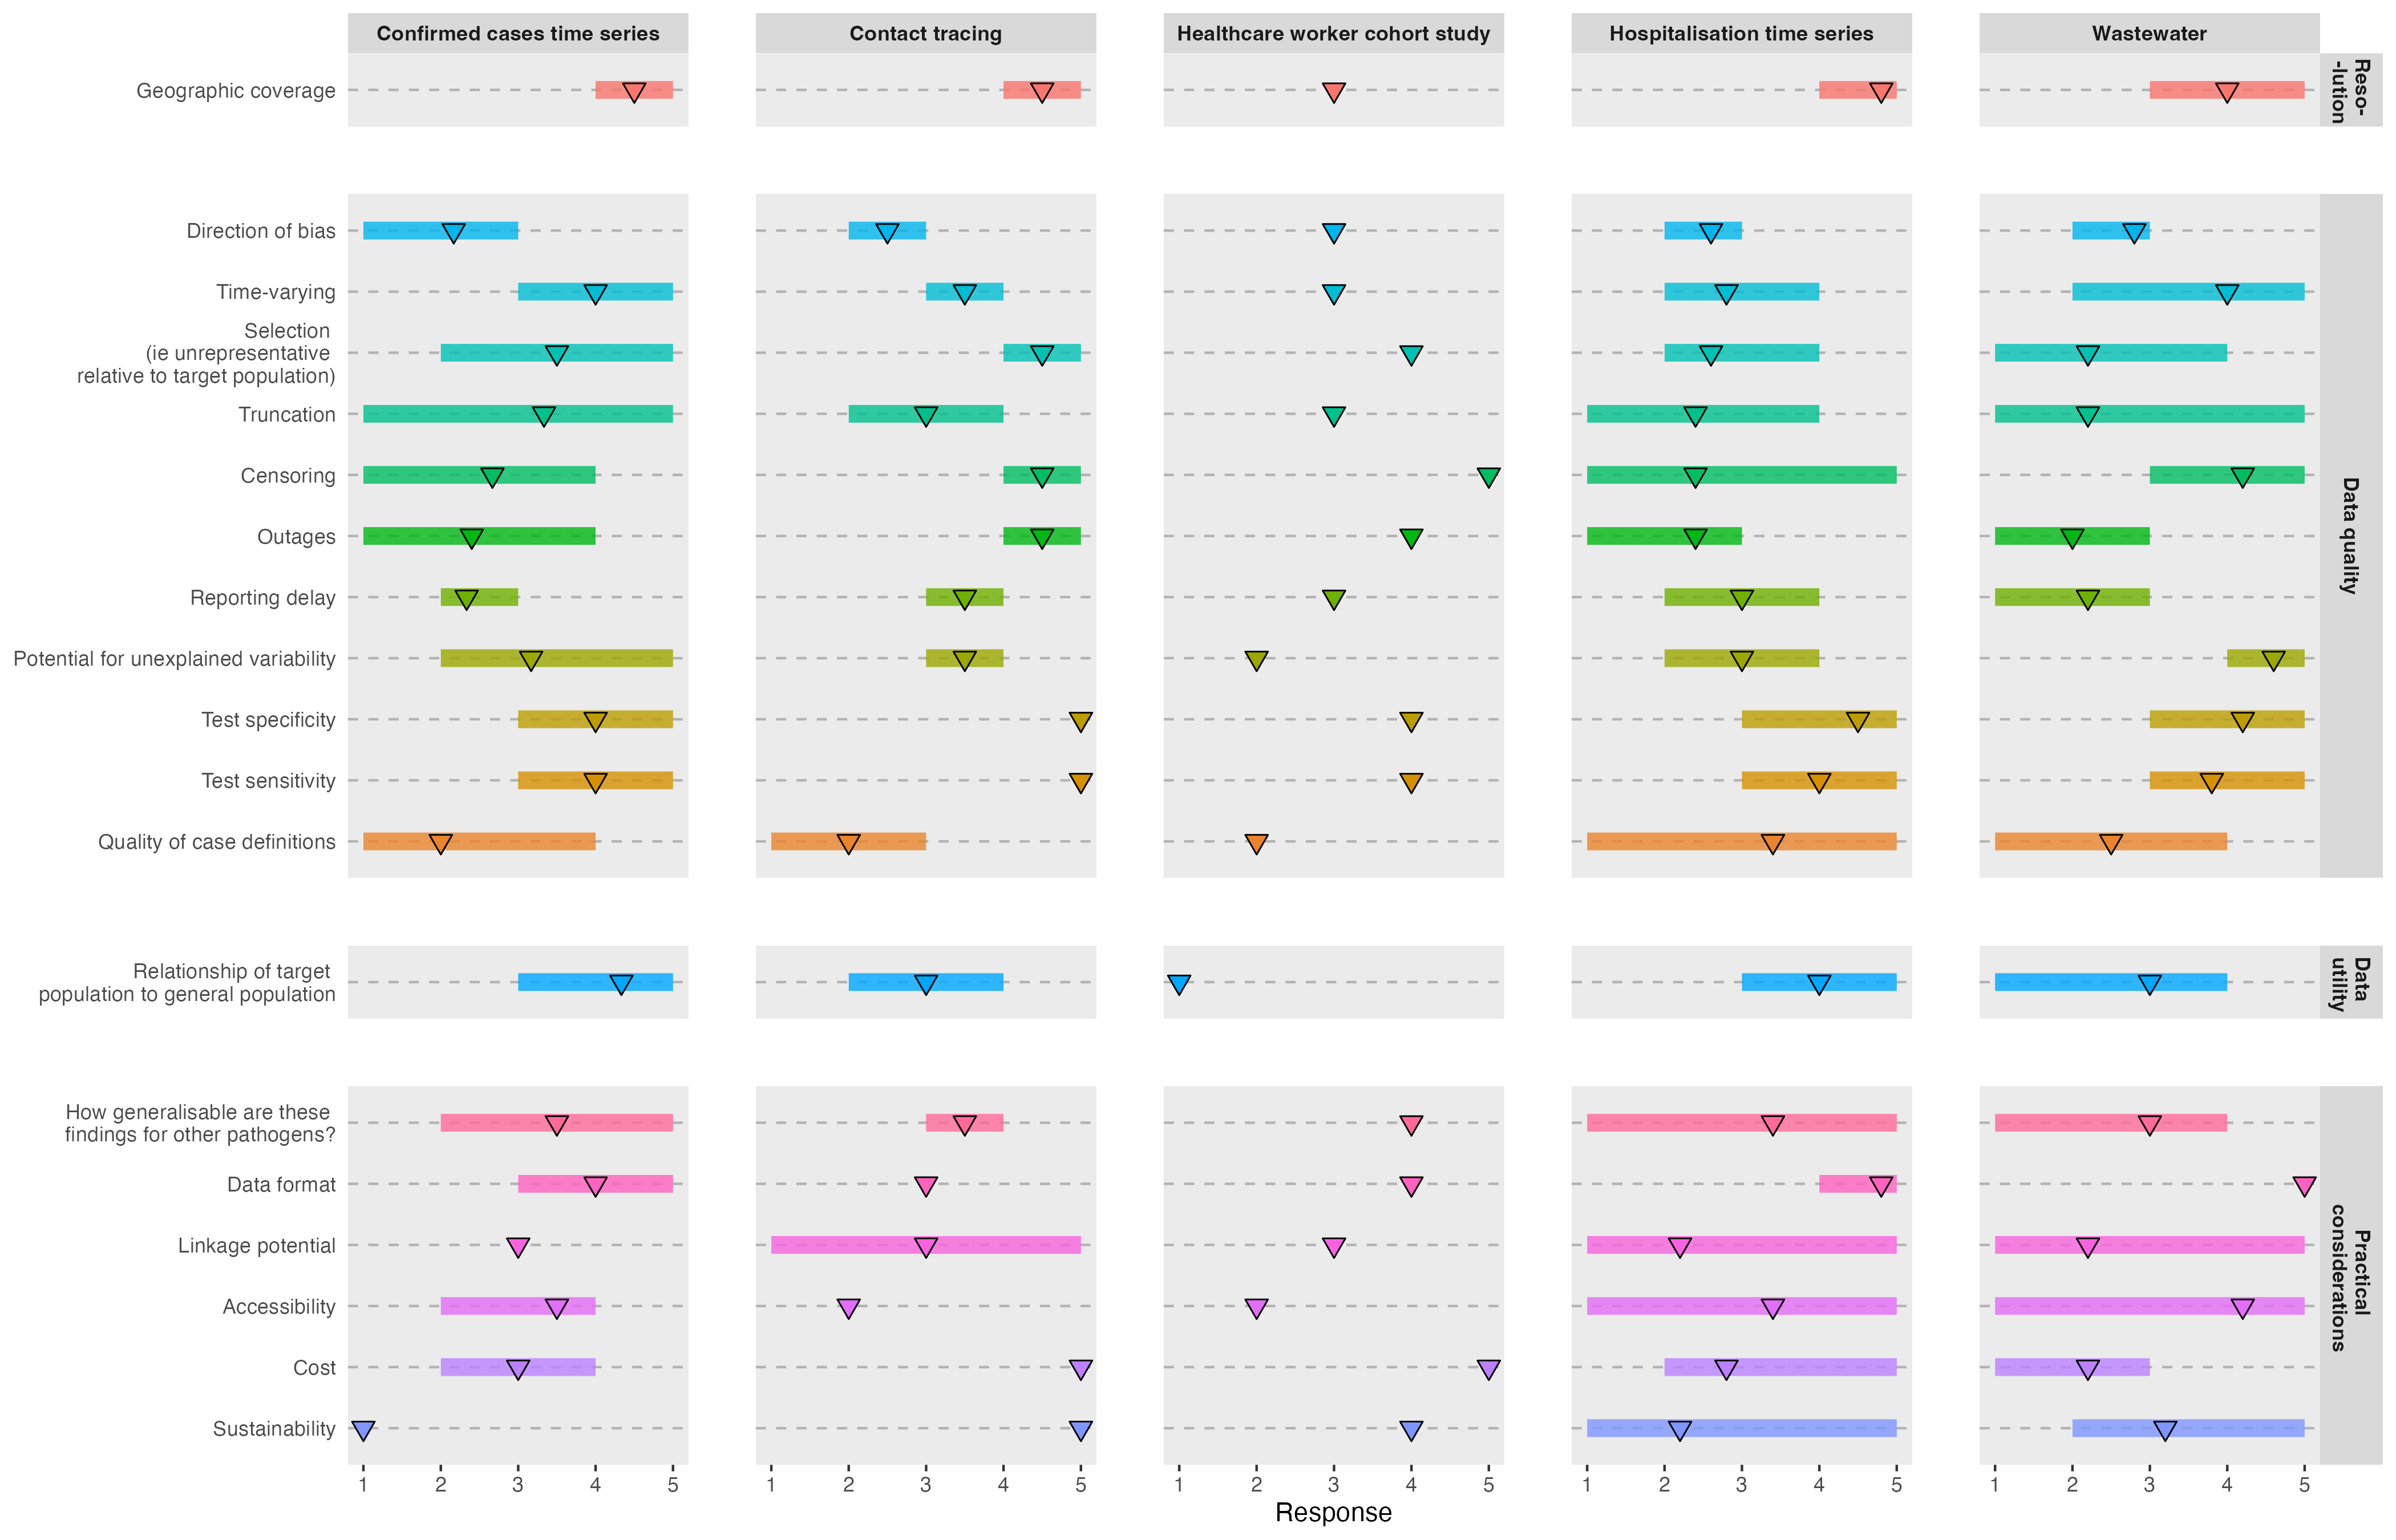
\includegraphics[width=1\linewidth]{supplement_figures/survey_responses_3.png}
\centering
\caption{Selected data characteristics from the survey, showing responses related to confirmed cases time-series, contact tracing, healthcare worker cohort study, and wastewater. The y-axis represents specific data characteristics, while the x-axis indicates the response range on a 5-point scale, where 1 corresponds to a low level and 5 to a high level. The lower triangles present the average response for each data characteristic.}
\label{survey_responses}
\end{figure}
    \begin{figure}[H] 
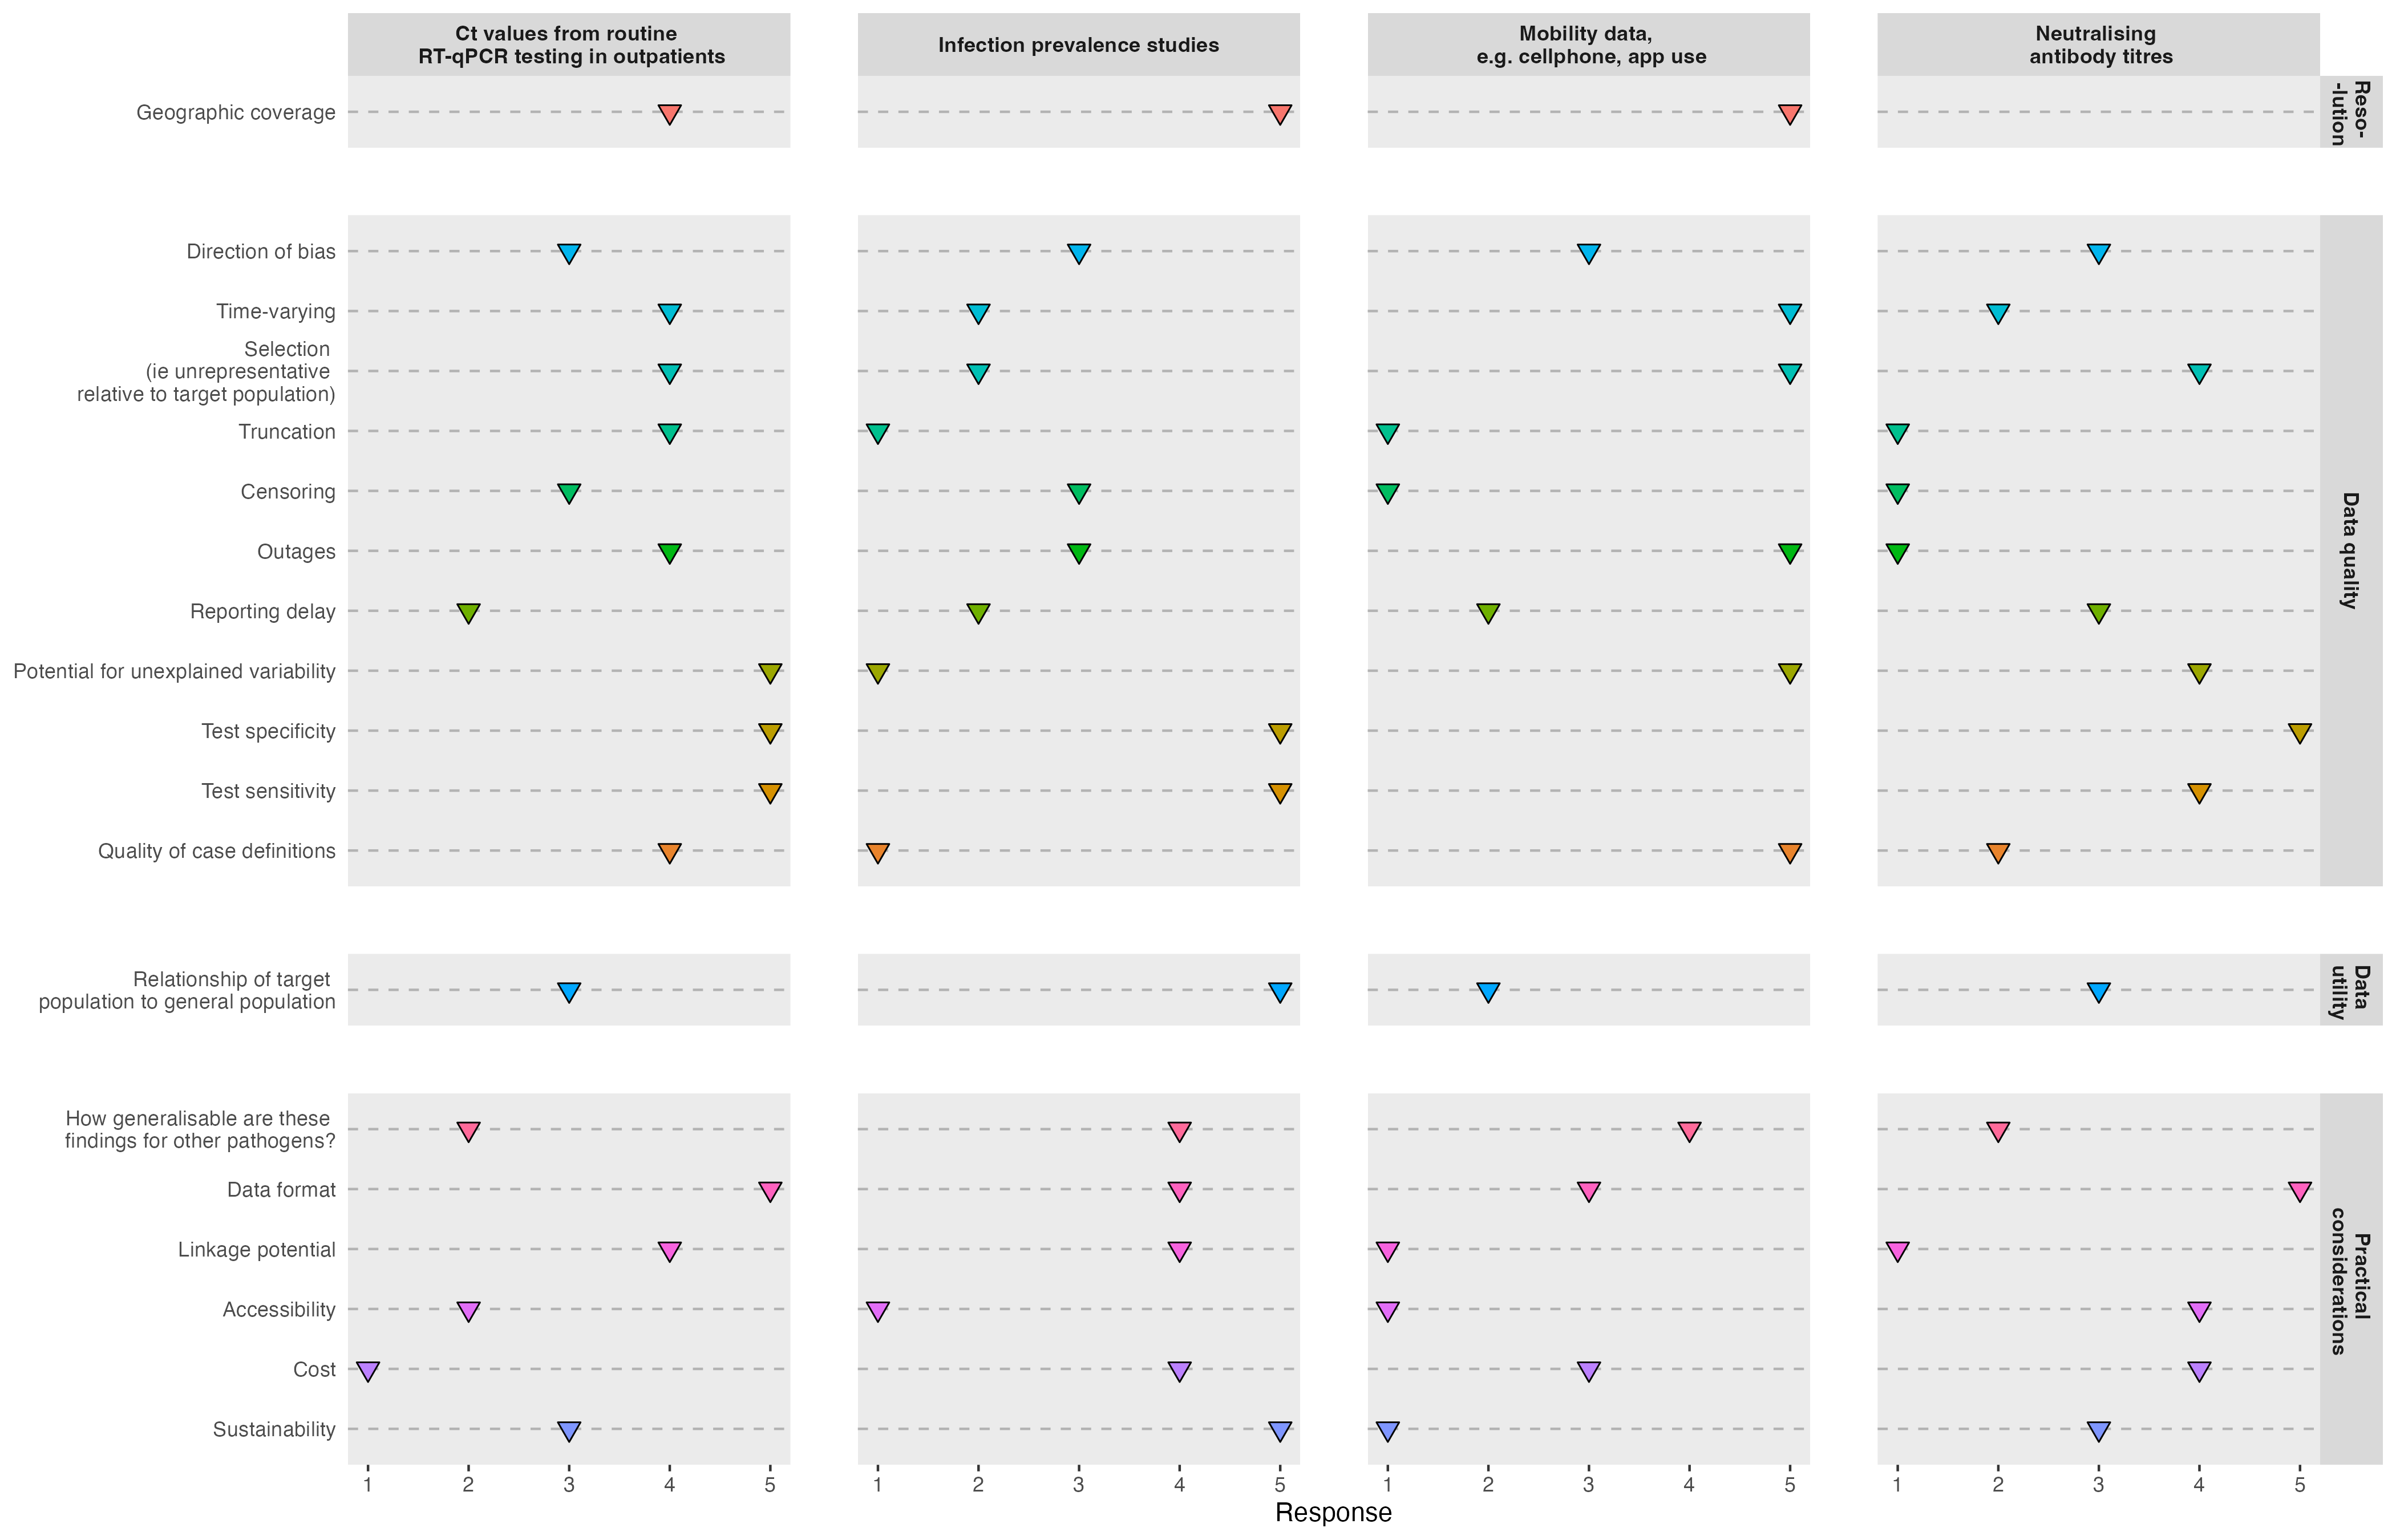
\includegraphics[width=1\linewidth]{supplement_figures/survey_responses_4.png}
\centering
\caption{Selected data characteristics from the survey, showing responses related to Ct-values from routine RT-qPCR testing in outpatients, infection prevalence studies, mobility data, and neutralising antibody titers. The y-axis represents specific data characteristics, while the x-axis indicates the response range on a 5-point scale, where 1 corresponds to a low level and 5 to a high level. The lower triangles present the average response for each data characteristic.}
\label{survey_responses}
\end{figure}
\end{landscape}


\subsection{The complete questionnaire}
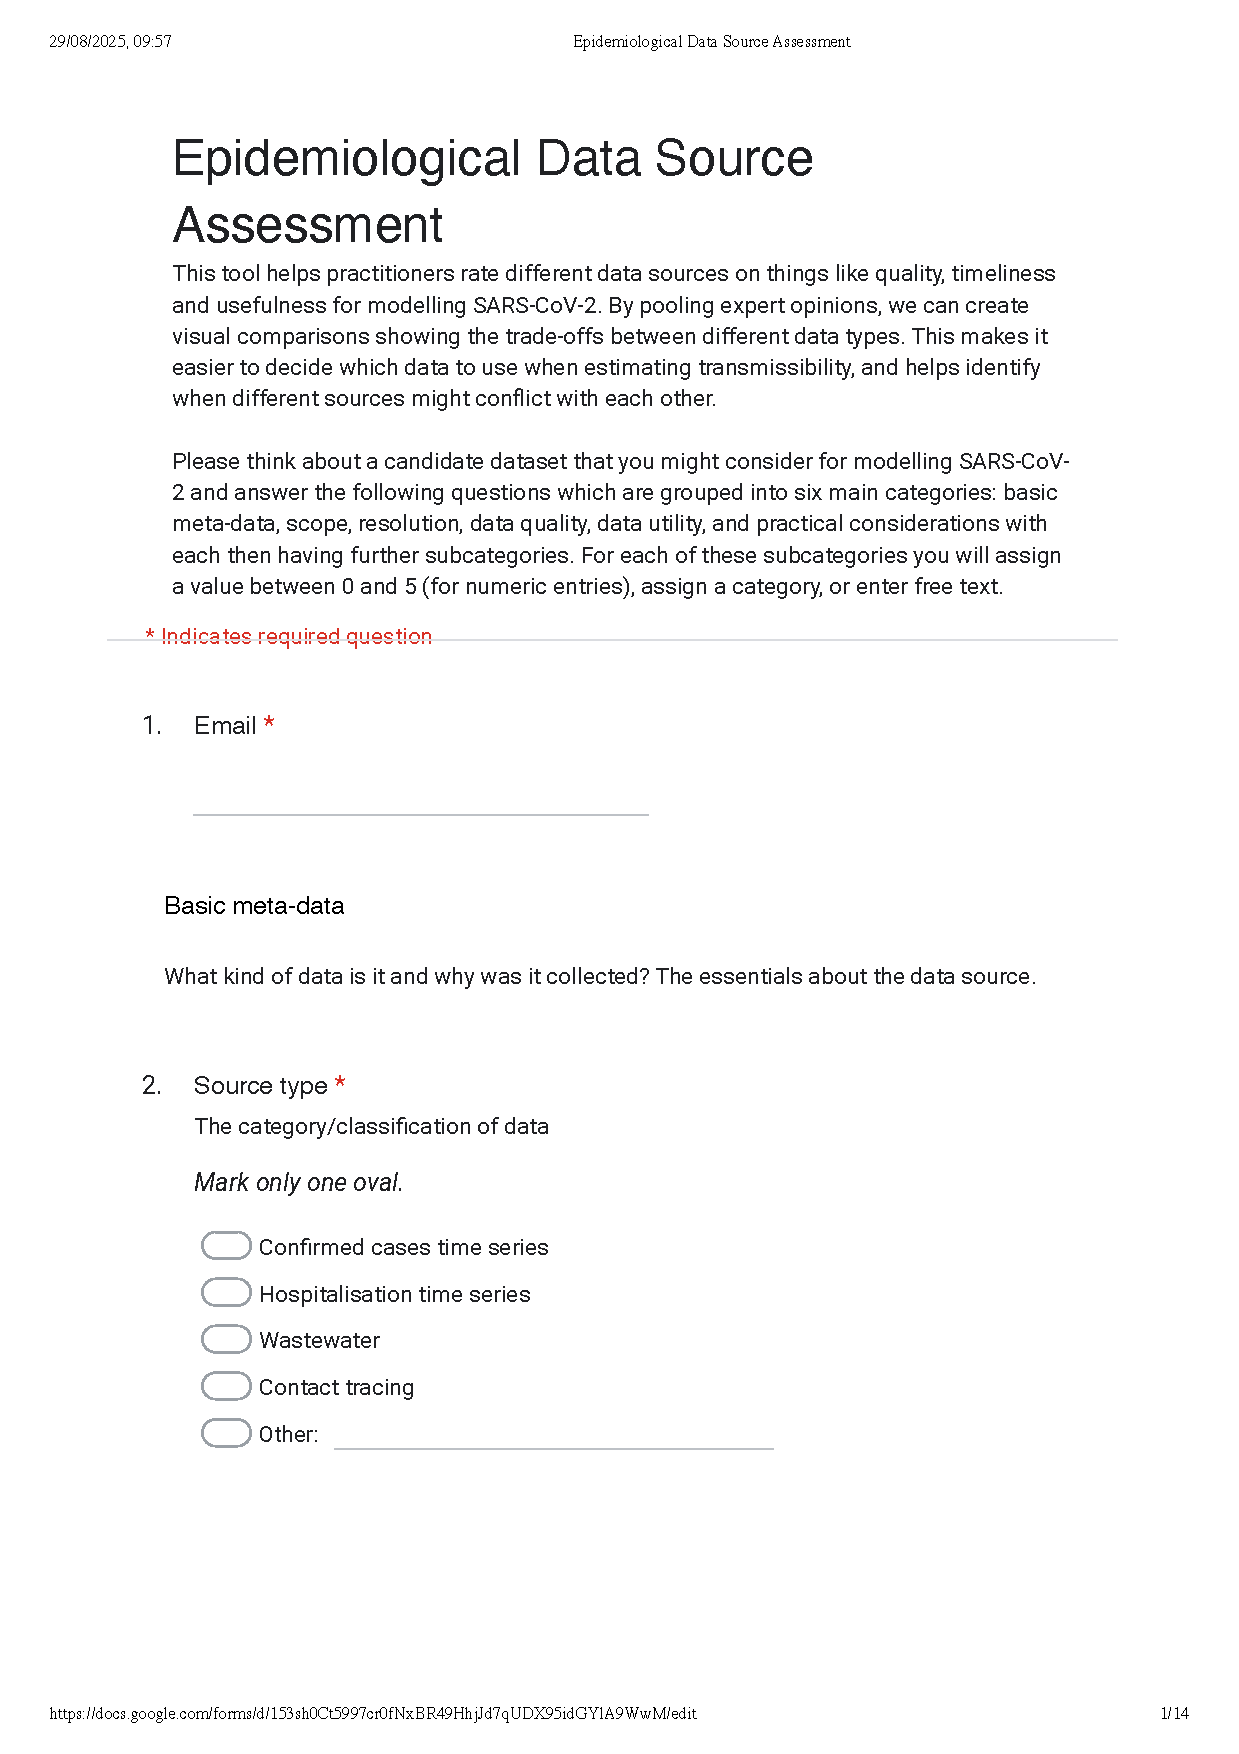
\includepdf[pages=-]{supplement_figures/survey.pdf}



\section{Code availability}

\bibliographystyle{plainnat}
\bibliography{references,zotero-references}

\end{document}